\documentclass[%
 reprint,
 amsmath,amssymb,
 aps,
 pra,
]{revtex4-1}

\usepackage{graphicx}% Include figure files
\usepackage{dcolumn}% Align table columns on decimal point
%\usepackage{bm}% bold math
\usepackage{fullpage}
\usepackage{epsfig}
\usepackage{amsmath}
\usepackage{amsthm}
\usepackage{amsfonts}
\usepackage{amssymb}
\usepackage{float}
\usepackage{pstricks}
\usepackage{cancel}
\usepackage{lipsum}
%\usepackage[nottoc,numbib]{tocbibind} %Uncomment for bibliography to be its own numbered section
\usepackage{units}
\usepackage{listings}
\usepackage{xfrac}

\graphicspath{{./plots/}}

\begin{document}

\preprint{APS/123-QED}

\title{\textbf{Lab Report: X-Ray Diffraction and Florescence} \\ \small{An Investigation of Characteristic Transitions of Atoms}}
\author{Joshua LaBounty}
\author{Thomas Krahulik}
\affiliation{Stony Brook University --- PHY 445}

\date{\today}

\begin{abstract}
In this experiment, we explore the characteristic x-rays produced by various elements and use them to probe the crystal structure of cubic Alkali halide crystals. Using an electron gun, we excite the characteristic transitions of a number of elements ranging in $Z$ from Lithium ($Z = 3$) to Uranium ($Z = 92$). We then use this data to recreate Moseley's Plot of Frequency vs. Atomic Number, and verify his eponymous empirical law. We then use these x-rays to probe the crystal structures of LiF, KCl, and NaCl and determine their lattice spacing. We find that our experimental lattice spacings are consistent with the known values.
\end{abstract}
\maketitle

\section{Introduction}

In October of 1895, Wilhelm R\"{o}ntgen was undertaking a study of cathode rays when he observed something highly unusual. A florescent screen set a few meters away from his apparatus was glowing\cite{xray_history}, far beyond the maximum distance a cathode ray could cause florescence ($\approx 10~cm$). This anomalous glow caught his attention, and he spent a frantic six weeks in the laboratory examining his findings and exploring this new radiation. He emerged with a photograph of the bones in his wifes hand and announced to the world his discovery of a new type of radiation, the "x-ray"\cite{rontgen_paper, 50years}, caused by cathode rays impacting on a material object. These rays caught the world by storm, and a flurry of new research into their properties quickly ensued.

A few years after their discovery Max von Laue, a student of Max Planck, became interested in studying the diffraction of x-rays. He had formulated a theory which described the diffraction behavior of light in parallel planes, and theorized that he could use the regular structure of crystal lattices to study the diffraction of x-rays\cite{xray_history}. His experiments quickly showed that x-rays which passed directly through crystals emerged diffracted into a pattern of concentric circles. This result, which earned Laue the Nobel Prize in 1914, simultaneously demonstrated the wave properties of x-rays and birthed an entirely new discipline --- x-ray crystallography\cite{laue}. 

While Laue had been primarily interested in using the diffracting crystals as a way to explore the properties of x-rays, many scientists soon realized that they could do exactly the opposite. In particular, William Lawrence Bragg and his father William Henry Bragg became interested in how a specific incidence of Laue Diffraction could be used to study the structure of crystalline materials. They found that x-rays which diffracted off of the surface of a crystal would exhibit interference patterns with maxima given by the following relation (for a derivation, see Appendix \ref{section:bragg_derivation}):
\begin{gather}\label{eq:bragg}
	d\sin\theta = n \lambda
\end{gather}
where $n = 1,2,3...$, $\lambda$ the wavelength of the characteristic x-ray, and $d$ the distance between the planes of the crystal. They selected for certain x-ray wavelengths by using narrow band filters, so the only variable in their measurements was $d$. This result earned the Bragg's the Nobel Prize in 1915.

The Bragg's observed that these diffraction patterns were only consistent so long as the material which produced the x-rays stayed consistent between experiments. If the material of the anode in their x-ray tubes was changed, the pattern they observed from the same crystal would also be changed, indicating that the wavelength of the x-ray had also changed. This peculiarity is what prompted Henry Moseley to begin his investigation of the x-ray spectra of different elements\cite{xray_history, moseley}. % By taking the x-ray spectra from the same crystal, but with different anodes producing the x-rays, Moseley was able to determine an empirical law which linked the atomic number of an element with the frequency of its characteristic x-rays.

The phenomenon responsible for the characteristic x-rays of different elements is x-ray fluorescence. When an atom is struck by an incident x-ray, the energy of the incoming photon excites an electron to a higher energy, leaving a hole in a lower energy level of the atom. When the excited electron returns to the lower state, the additional energy from the original incident radiation is released by the emission of a new x-ray photon. The x-ray generated by this fluorescence has a distinct wavelength associated with the energy transition that the electron undergoes. The collection of wavelengths emitted by an atom are known as the characteristic lines of that atom.

Noticing the variation in characteristic lines for different elements, Moseley tried to find some relationship between an element and the x-ray photons it emitted in x-ray fluorescence. Moseley found that the frequency (and therefore energy) of the x-rays was proportional to the square of an effective nuclear charge, $Z_{eff} = Z - \sigma$ of the atom. $\sigma$ is a screening factor that lowers the nuclear charge "observed" by the excited electron that arises due to the presence of additional electrons\cite{moseley}. This relationship is defined by Moseley's Law in Eq.~\ref{Eq:MLaw}. 

\begin{equation}\label{Eq:MLaw}
E = h\nu = A Z_{eff}^{2} = A (Z - \sigma)^2
\end{equation}

The parameters $A$ and $\sigma$ depend on which type of transition the excited electron undergoes. Moseley used the Bohr model of the atom to describe these transitions. In the Bohr model of the atom, the energy of an electron determines what energy level it occupies. These energy levels are labeled as $n = 1, 2, 3, etc.$ or the K, L, M, etc. shells. When an excited electron transitions back to one of these shells it determines which series of characteristic x-ray is emitted. For example, an electron transitioning to the $n = 1$ energy level (K shell) emits an x-ray of the K series. The series can be further identified by the location of the electron when it is excited. An electron lowering from $n = 2$ to $n = 1$ emits an x-ray of the $K_{\alpha}$ series, one lowering from $n = 3$ to $n = 1$ emits an x-ray of the $K_{\beta}$ series, etc. An experimental analysis of Moseley's Law will display these series as distinct linear relationships on a plot of $Z$ vs $\sqrt{\nu}$. Using the Bohr model of the atom does not account for the fine structure splitting of energy levels, which becomes evident in small discrepancies between theory and experiment, but the model acts as a sufficient starting point for understanding the origin of Moseley's Law.

\section{Review of Previous Work}

As soon as they were discovered, measurements of x-rays became standard tools in the handbook of the experimental physicist, as well as the chemist and medical doctor. In particular, x-ray diffraction and florescence measurements were particularly useful for probing the composition of materials down to the atomic scale. 

The Braggs pioneered the investigation of the crystal structure of simple crystals\cite{bragg, xray_history}, while many others built upon their work to examine the crystal structures of complex molecules. Less than 50 years after Laue's discovery, the crystal structures of DNA\cite{dna1, dna2}, Insulin\cite{insulin}, and many other important biological molecules were discovered\cite{scatter_medicine_1, scatter_medicine_2}. Recently, imaging of entire living cells with x-rays has also become feasible, opening new doors to understanding the flow of chemicals within the cells themselves\cite{whole_cells}. Measurements of Bragg scattering have also become a favorite of undergraduate physics laboratories, and thus the results of the scattering experiments have been replicated many times over\cite{scatter_lab_1, scatter_lab_2, jensen}. Laue and Bragg measurements of crystal structure, like those performed in this lab, are still used in condensed matter laboratories to probe the structures of new crystals in a search for high temperature superconductors\cite{aronson, aronson2}.

Because each element has its own unique set of characteristic x-rays, x-ray florescence is an important tool in the identification of unknown materials. Before his study was even complete, Moseley was applying his findings to the identification of unknown samples. With a single measurement, he was able to show that the 'element' Celtium, isolated by Carl Auer von Welsback, was actually a mixture of lutecium and ytterbium\cite{xray_history}. Many measurements of these characteristic x-rays have been undertaken over the years, and their energies are known to many decimal places\cite{database1, database2}. Measurements like the ones we do in this report were crucial to establishing these known values.

Because the strength of the emission lines is also dependent on the concentration of the element in the sample\cite{miller}, it is also possible to determine relative concentrations of elements and not simply their presence. This allows the measurement of trace elements in samples to a great deal of precision, which has applications in a wide range of fields. It can be used in the identification of counterfeit works of art\cite{art1, art2, art3}, as the composition of available pigments differed vastly throughout history. Floresence studies are also used in determining the diet of ancient hominids from the composition of their bones\cite{art3, arch1, arch2, traces}.

\section{Experimental Setup}

\subsection{X-Ray Florescence}

The apparatus used in our measurements of x-ray florescence consists primarily of two components, an electron gun and a solid state detector, as shown in Figure \ref{fig:xrf_setup}. The electron gun operates by running current through a filament in a potential. As the filament heats, electrons are 'boiled off' (a process known as thermionic emission) and are accelerated towards the anode by the potential. Some of the electrons strike the anode, but the rest escape through the opening into a collimated beam of particles. The energy of these electrons is defined by their accelerating voltage: $E_{e^-} = qV$, while their number is defined by the current. These electrons impact the sample and cause it to emit photons, which are then picked up by the detector. 

\begin{figure}[H]
	\centering
	\includegraphics[width=0.25\textwidth]{xrf_experiment.png}
	\caption{Experimental Setup used in XRF portion of the experiment.}
	\label{fig:xrf_setup}
\end{figure}

The detector is a Silicon p-i-n diode manufactured by Amptek. Photons incident on the detector are first met with a window made of Beryllium, which is opaque to photons with $E_\gamma <1~keV$. Photons with sufficient energy pass through and deposit their energy in the sensitive volume of the detector, ionizing the silicon atoms and creating a number of electron-hole pairs. A bias voltage across the diode causes these electron/holes to flow and be read into the detector as a pulse of charge, whose magnitude is directly proportional to the energy which was deposited in the detector by the photons. This pulse is passed through an amplifier, which is then passed into the multi-channel analyzer (MCA), and then from there into the computer system. From there, the information is saved in a format which can be read into our data analysis software, ROOT. This software is developed and maintained by scientists at CERN, and contains many useful fitting and histogram manipulation packages. We also performed independent cross checks of its $\chi^2$ minimization techniques, which can be found in Appendix \ref{section:root}.

\subsection{X-Ray Diffraction}

This apparatus consists of three primary components: the x-ray source, the goniometer, and the detector. The x-ray source uses the same method of x-ray production as the setup detailed above. However, instead of switching the samples out to change the characteristic x-rays of the system, here the target sample for the electrons is kept constant, and is composed of copper. These x-rays are collimated by sheets of lead with small openings and then allowed to stream freely towards the sample. The second portion of the experiment is the goniometer, which keeps the relative angle of the sample and the detector constant: $\theta_{\text{detector}} = 2\theta_{\text{sample}}$ (relative to $\theta = 0$ defined by the path of the undiffracted x-rays). The x-rays which are diffracted off of the sample then enter the detector. This detector differs from the previous version in that it is a Geiger-Muller detector. 

\begin{figure}[H]
	\centering
	\includegraphics[width=0.3\textwidth]{xrd_experiment.png}
	\caption{Experimental Setup used in XRD portion of the experiment.}
	\label{fig:xrd_setup}
\end{figure}

In this detector, a low-pressure inert gas is encased in a cavity. At either end of this cavity is an anode and a cathode, across which a high voltage is applied. When ionizing radiation enters the cavity, molecules of the gas become ionized. The electron and nucleus then fly in opposite directions, accelerated towards the anode and cathode respectively. As the electron travels through the gas, it causes the ionization of subsequent electrons in an 'avalanche', effectively multiplying its own signal. This flow of liberated electrons creates a fast pulse of charge which is read by the tube as a single event. After the pulse is complete, the atoms in the gas return to their neutral state and the detector is ready to detect another event. The time that the pulse takes is known as the \textit{dead time} of the detector, as events can only be detected one at a time, and the detector is effectively dead until the initial pulse is complete. 

This pulse of current is first sent into a pre-amplification system and from there into a counter, rate meter, and oscilloscope. The oscilloscope serves only to show a visual representation of the pulses, and we will use it to characterize the dead time of our detector. The rate meter gives us a measure of the counts/second the detector is seeing, and warns if the detector is becoming saturated (i.e. events are coming in too quickly to all be counted). The counter simply records the number of events in a specified amount of time. We will compare the output from the counter across a wide range of angles in order to determine the number flux of photons at each angle. We recorded this data manually and input it into an excel spreadsheet, so it could be plotted in real time. In order to perform our final analysis, this spreadsheet was converted into a \verb|.txt| file which we read in to ROOT.

\section{Measurements}

\subsection{X-Ray Florescence}

\begin{figure}[H]
	\centering
	\includegraphics[width=0.4\textwidth]{InBinnedSpectrum.png}
	\caption{X-Ray Fluorescence Spectrum for Indium}
	\label{Fig:InXRFSpec}
\end{figure}

Before performing an analysis of x-ray fluorescence, we had to calibrate the energy scale of the MCA to determine the conversion between the channel number ($n$) of a detected photon and its energy. In order to perform this calibration, x-ray fluorescence spectra were collected for various samples with known energy peaks. Fig.~\ref{Fig:InXRFSpec} displays an example spectrum with fitted peaks.

Each peak on one of these spectra was fit with a Gaussian distribution to find the mean value of the peak. This mean value was stored as the bin number corresponding to the peak of known energy provided by external sources. We collected corresponding energies and bin numbers for several samples of different elements to generate the energy vs bin number plot in Fig.~\ref{Fig:Evsbin}.

\begin{figure}[H]
	\centering
	\includegraphics[width=0.4\textwidth]{EvsBin.png}
	\caption{Energy vs Channel Number Calibration Plot}
	\label{Fig:Evsbin}
\end{figure}

The linear fit on this plot provided us with the energy calibration in Eq.~\ref{eq:ECalib}.
\begin{gather}\label{eq:ECalib}
	E = 0.0245644n - 0.0545754
\end{gather}

With this calibration, we could then calculate the energies of peaks in our x-ray fluorescence spectra. As previously discussed, peaks in the energy spectra for different elements were fit with a Gaussian distribution to find the mean value of the peaks which we converted to energy using our calibration. Each energy peak we analyzed corresponded to the $K_{\alpha}$, $K_{\beta}$, etc. transitions which we could confirm with outside sources. For each type of transition, we could record the atomic number, $Z$ and the energy of the emitted x-ray photon for several samples. For a more clear analysis of Moseley's Law, we derived Eq.~\ref{Eq:MLaw} in the following manner to obtain the linear relationship expressed in Eq.~\ref{Eq:MLawLinear}.

\begin{align*}
A(Z - \sigma)^{2} &= E\\
A(Z - \sigma)^{2} &= h \nu\\
Z - \sigma &= \sqrt{\frac{h}{A}}\sqrt{\nu}
\end{align*}
\begin{equation}\label{Eq:MLawLinear}
Z = \sqrt{\frac{h}{A}}\sqrt{\nu} + \sigma
\end{equation}

As demonstrated by Eq.~\ref{Eq:MLawLinear}, plotting data of $Z$ vs. $\sqrt{\nu}$ should yield a linear relationship with a slope of $\sqrt{\sfrac{h}{A}}$ and an offset equal to the screening parameter $\sigma$. We performed this analysis for many samples of different elements to generate the plot in Fig.~\ref{Fig:MLawPlot}.
\begin{figure}[H]
	\centering
	\includegraphics[width=0.48\textwidth]{MoseleyLawPlot.png}
	\caption{Plot Displaying Moseley's Law for $K_{\alpha}$, $K_{\beta}$, $L_{\alpha}$, $L_{\beta}$, and $L_{\gamma}$ Transitions}
	\label{Fig:MLawPlot}
\end{figure} 

The data for each series ($K_{\alpha}$, $K_{\beta}$, etc.) of transition was fit to a line to observe its consistency with Moseley's Law. Table~\ref{Tab:MLawData} presents the parameters determined from each of the linear fit functions while Table~\ref{MLawChiSq} shows the reduced chi-squared values for each of these fits.
\begin{table}[htbp]
	\begin{center}
		\begin{tabular}{|c|c|c|c|}
			\hline Transition & $\sqrt{\frac{h}{A}}$ ($ 10^{-8} s^{\frac{1}{2}}$)  & $A$ ($10^{-18} J$) & $\sigma$ \\
			\hline $K_{\alpha}$ & $1.964 \pm 0.009$ & $1.717 \pm 0.016$ & $1.621 \pm 0.166$ \\
			\hline $K_{\beta}$ & $1.824 \pm 0.007$ & $1.991 \pm 0.015$ & $2.240 \pm 0.141$ \\
			\hline $L_{\alpha}$ & $4.668 \pm 0.056$ & $0.304 \pm 0.007$ & $7.470 \pm 0.814$ \\
			\hline $L_{\beta}$ & $3.959 \pm 0.051$ & $0.423 \pm 0.011$ & $13.126 \pm 0.754$ \\
			\hline $L_{\gamma}$ & $3.491 \pm 0.074$ & $0.544 \pm 0.023$ & $16.215 \pm 1.235$ \\
			\hline
		\end{tabular}
	\end{center}
	\caption{Calculated Parameters in Moseley's Law for Each Type of Shell Transition}
	\label{Tab:MLawData}
\end{table}

\begin{table}[htbp]
	\begin{center}
		\begin{tabular}{|c|c|}
			\hline Transition & $\chi_{red}^2$ \\
			\hline $K_{\alpha}$ & $0.1916$ \\
			\hline $K_{\beta}$ & $0.31316$ \\
			\hline $L_{\alpha}$ & $0.138634$ \\
			\hline $L_{\beta}$ & $1.1486$ \\
			\hline $L_{\gamma}$ & $0.405954$ \\
			\hline
		\end{tabular}
	\end{center}
	\caption{Calculated Parameters in Moseley's Law for Each Type of Shell Transition}
	\label{Tab:MLawChiSq}
\end{table}

The low $\chi_{red}^2$ values for each of these fits demonstrates that the x-ray fluorescence spectra collected during the experiment do behave according to Moseley's Law. The next step is to test the experimentally measured parameters in Table~\ref{Tab:MLawData} against theoretically expected values.

\subsection{X-Ray Diffraction}

\subsubsection{Analysis of the Detector}

\begin{figure}[H]
	\centering
	\includegraphics[width=0.4\textwidth]{xrd_setup_investigation.png}
	\caption{Investigation of the properties of the x-ray diffraction GM detector and x-ray source}
	\label{fig:xrf_setup_investigation}
\end{figure}

To begin this experiment, we needed to characterize the behavior of the detector with respect to the Voltage and Current of the x-ray source, the Voltage of the detector, and the gain settings of the signal amplification. To do this, we positioned the detector with no crystal at a slight angle $\approx 2^\circ$ and performed a series of measurements in which we fixed all but one of these variables and varied the other. A subset of these plots can be seen in Figure \ref{fig:xrf_setup_investigation}. These plots helped to inform our decision for the detector/source settings used in the main measurements.

\begin{figure}[H]
	\centering
	\includegraphics[width=6cm]{dead_time.png}
	\caption{Illustration of the dead time of a Geiger-Muller tube. Image courtesy of Wikimedia Commons.}
	\label{fig:dead_time}
\end{figure}

One important quantity that we needed to determine is the dead time of the detector. Using the oscilloscope readout, we determined the dead time of our detector at the settings we would be using for our subsequent data taking. We set the discriminator fine gain to $1.0$, the discriminator course gain to $\sfrac{1}{16}$, and the voltage of the detector to $V_{det} = 450~V$. At these settings, we observed pulses of similar shape to the one shown in Figure \ref{fig:dead_time}. We measured the width of those pulses in $t$ using the lines on the oscilloscope screen and determined them to be $\tau_{dead} = 0.1 \pm 0.01~ms$. This means that saturation count rate for our detector would be $1/\tau_{dead} = 10,000 \pm 1,000~\text{photons}/s$. Thus, during the subsequent experiments, we took care to keep our peak count rate under that value, or else we risked not being able to distinguish between closely spaced peaks.

Using this dead time determination alongside the data in Figure \ref{fig:xrf_setup_investigation}, we determined the settings for the detector which would optimize our particle count at the peaks to be just under the limit imposed by the dead time. The settings we chose were: $I_{source} = 80~mA$, $V_{source} = 20~kV$, $V_{detector} = 450~V$, Fine Gain$ = 1.0$, and Course Gain$ = \sfrac{1}{16}$. We found that these numbers produced counts which were high enough to get a good resolution of the peaks, but not high enough to saturate the detector.

\subsubsection{Diffraction Spectra}

After we characterized the detector, we set out to measure the diffraction spectra of each of the three crystals: KCl, LiF, and NaCl. We placed each crystal in the mount on the goniometer and aligned the system. In particular, we ensured that the crystal was vertical, that the collimated beam would just skim over the surface of the crystal at $\theta = 0^\circ$, and that an angular change in the detector position of $\theta_{det}$ corresponded to a change in the angle of the crystal of $\theta_{cry} = \theta_{det}/2$. 

We set the x-ray source to $I_{source} = 80~mA$ and $V_{source} = 20~kV$ for all of these scans. We scanned in $2.5^\circ$ increments outside the regions where there were diffraction peaks present, and in $0.5^\circ$ increments within the regions of interest. We estimated our systematic error in each of these measurements to be $0.25^\circ$, accounting for the 'play' in the gear system as well as for our error in the placement of the detector. At each point, we took three measurements of 10 seconds each. Poisson tells us that if we observe $N$ counts in the measurement, the error in the measurement is $\sqrt{N}$. Therefore the overall error in our measurement is $\delta N =\bar{N}\sqrt{N_1/N_1^2 + N_2/N_2^2 + N_3/N_3^2}$. The spectra we measured for LiF and KCl can be seen in Figures \ref{fig:LiF} and \ref{fig:KCl} below:

\begin{figure}[H]
	\centering
	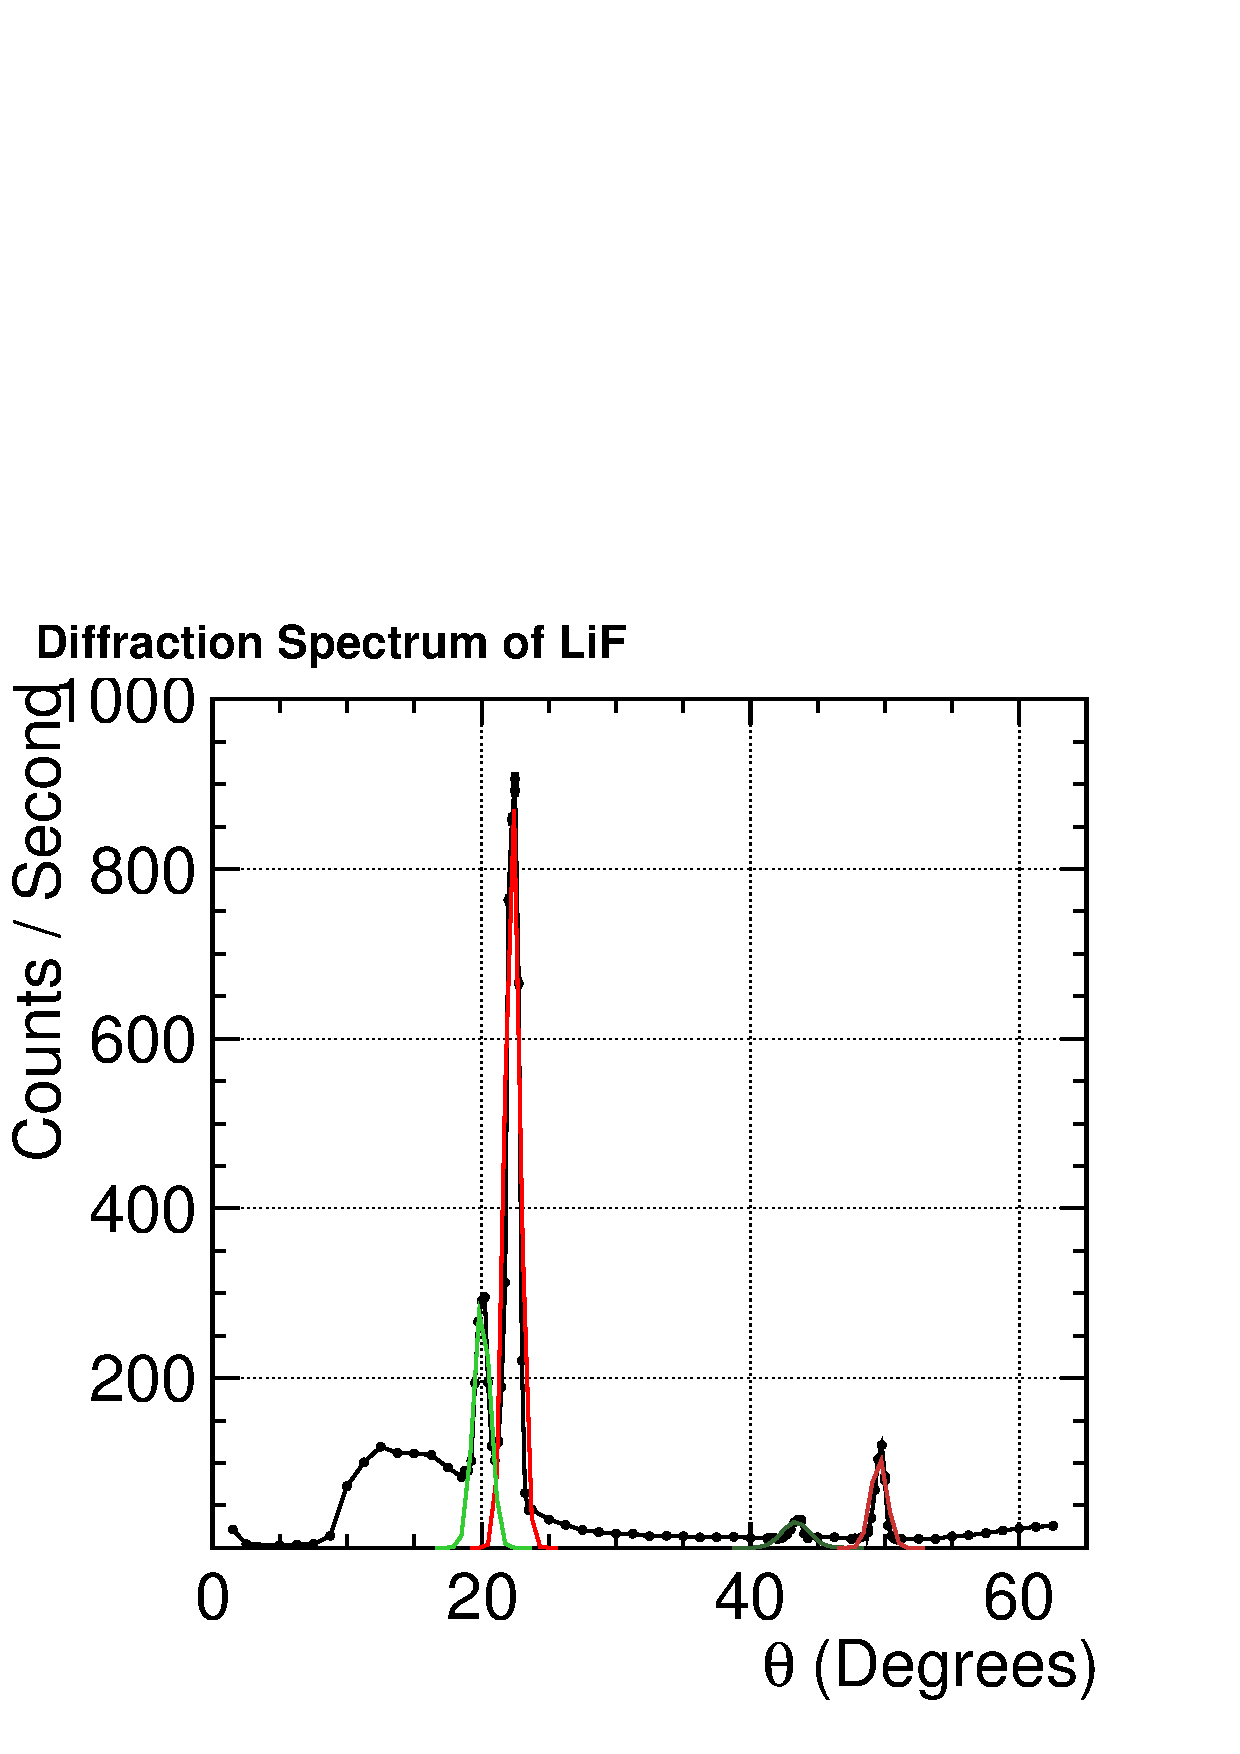
\includegraphics[width=0.4\textwidth]{Diffraction_LiF.png}
	\caption{Angular diffraction of Lithium Fluoride. Here, $\theta$ refers to the angle of the crystal, so the overall angular displacement of the detector is $2 \theta$.}
	\label{fig:LiF}
\end{figure}

\begin{figure}[H]
	\centering
	\includegraphics[width=0.4\textwidth]{Diffraction_KCl.png}
	\caption{Angular diffraction of Potassium Chloride. Here, $\theta$ refers to the angle of the crystal, so the overall angular displacement of the detector is $2 \theta$.}
	\label{fig:KCl}
\end{figure}

From these Figures, we observe two key features. We first can see that there is a bremsstrahlung spectrum which underlays all other features, starting at $\theta \approx10^\circ$ and extending out to the edge of the graph. At the far end ($\theta > 55^\circ$), we enter into a region where x-rays from the source start to enter the detector without scattering off of the crystal (simply due to the geometry of our setup). This causes these points to be artificially higher than the bremsstrahlung background would otherwise indicate. The second feature, and by far the more interesting, is the sets of two peaks beginning shortly after the bremsstrahlung spectrum. These are the characteristic $K_\alpha$ and $K_\beta$ x-rays of the source's anode, composed of Copper, scattering off of the crystal structure of the sample according to Bragg's Law, with $n = 1,~2,~3,...$ and with an as yet unknown lattice spacing. Using the data gathered above, in concert with the known $K_\alpha$ and $K_\beta$ values, we can determine the experimental values for the lattice spacing:
\begin{gather}
	2d\sin{\theta} = n\lambda \rightarrow d = \frac{n\lambda}{d\sin{\theta}} \nonumber \\
	\downarrow E_\gamma = \frac{hc}{\lambda} \rightarrow \lambda = \frac{hc}{E} \nonumber \\
	d = \frac{n (hc/E)}{2 \sin{\theta}} = \frac{nhc}{2E\sin{\theta}}
\end{gather}
The known energy values for copper are\cite{database1, database2}:
\begin{gather}
	K_\alpha = 8037.8 ~eV \nonumber \\
	K_\beta = 8905.29 ~eV \nonumber
\end{gather}
To each of the peaks in Figures \ref{fig:LiF}, we performed a fit consisting of a gaussian combined with a polynomial background using ROOT. From the parameters of this fit, we can extracted $\theta \pm \delta \theta$ and used them to construct the following table:
\begin{table}[htbp]
	\begin{center}
	\begin{tabular}{|r|r|r|r|r|r|l|}
		\hline
		n & $\theta$ (Deg) & $\delta \theta$ (Deg) & $K$ &  $d$ (nm) & \multicolumn{1}{r|}{$\delta d$ (nm)} \\ \hline
		1 & 20.0293 & 0.61075 & $\beta$ &  0.2034 & 0.005947 \\ \hline
		1 & 22.3206 & 0.55230 & $\alpha$ &  0.2032 & 0.004771 \\ \hline
		2 & 43.3667 & 1.01729 & $\beta$ &  0.2029 & 0.003814 \\ \hline
		2 & 49.5563 & 0.59909 & $\alpha$ &  0.2028 & 0.001808 \\ \hline
	\end{tabular}
	\end{center}
	\caption{Calculated lattice spacing for LiF.}
	\label{table:LiF}
\end{table}

\noindent From this we can see that the values we find for $d$ are consistent within the LiF crystal. The same analysis was undertaken for KCl and NaCl. Using this data, we obtain an average value for the lattice spacing for all three crystals:

\begin{table}[htbp]
	\begin{center}
	\begin{tabular}{|l|r|r|}
		\hline
		Crystal & \multicolumn{1}{l|}{$d_{avg}$ (nm)} & \multicolumn{1}{l|}{$\delta d_{avg}$ (nm)} \\ \hline
		\textit{LiF} & 0.2031 & 0.002179 \\ \hline
		\textit{KCl} & 0.3199 & 0.007197 \\ \hline
		\textit{NaCl} & 0.2875 & 0.005546 \\ \hline
	\end{tabular}
	\end{center}
	\caption{Average value of $d$ for all three crystals.}
	\label{table:d_average}
\end{table}

\noindent We will compare these values to their known values in the coming sections.

\section{Theoretical Model}

\subsection{X-Ray Florescence}

Moseley's Law as described in Eq.~\ref{Eq:MLaw} relates the energy ($E$) of x-ray fluorescence photons emitted from a sample to the square of an effective nuclear charge ($Z_{eff}^{2}$) with a parameter $A$. This parameter is dependent on which energy levels are involved in the electron transition in x-ray fluorescence. To determine a set of theoretical values for comparison with experimental results, we used the Bohr model of the atom as Moseley had done. For an electron that transitions from an excited state energy level $n_{i}$ to a lower energy level $n_{f}$, the $A$ parameter is defined by Eq.~\ref{Eq:RydbergParameter}, where the Rydberg constant $R = 1.097 \times 10^7~m^{-1}$, $h$ is Planck's constant, and $c$ is the speed of light in a vacuum.

\begin{equation}\label{Eq:RydbergParameter}
A = hcR \left( \frac{1}{n_{f}^{2}} - \frac{1}{n_{i}^{2}} \right)
\end{equation}

We calculated the theoretical values of $A$ for each of the different types of shell transitions and recorded these values in Table~\ref{Tab:RydParam}.

\begin{table}[htbp]
	\begin{center}
		\begin{tabular}{|c|c|c|c|}
			\hline Transition & $n_{i}$  & $n_{f}$ & $A (10^{-18} J)$ \\
			\hline $K_{\alpha}$ & $2$ & $1$ & $1.635$ \\
			\hline $K_{\beta}$ & $3$ & $1$ & $1.938$ \\
			\hline $L_{\alpha}$ & $3$ & $2$ & $0.303$ \\
			\hline $L_{\beta}$ & $4$ & $2$ & $0.409$ \\
			\hline $L_{\gamma}$ & $5$ & $2$ & $0.458$ \\
			\hline
		\end{tabular}
	\end{center}
	\caption{Calculated Parameters in Moseley's Law for Each Type of Shell Transition}
	\label{Tab:RydParam}
\end{table}

As previously mentioned, the Bohr model of the atom does not account for further quantum mechanical effects such as fine structure splitting. This means that the behavior of x-rays predicted by this model will show some deviation from experimental data.

\subsection{X-Ray Diffraction}

The hard sphere model of the atoms is a theory of crystal structure whose premise is that the atoms in the lattice can be treated as hard spheres directly in contact with one another. The distance between the crystal planes then simply becomes the sum of the radii of the two spheres. Pauling calculated these radii from an estimate of the effective nuclear charge of each ion\cite{hard_sphere2}, the results of which were compiled and modified slightly by R.D. Shannon\cite{hard_sphere}. Estimates of the spacing for our crystals from Snannon's tables can be seen in Table \ref{table:hardsphere_d} below:

\begin{table}[htbp]
	\begin{center}
	\begin{tabular}{|l|r|r|r|}
		\hline
		\textbf{Crystal} & \multicolumn{1}{l|}{\textbf{$r_1$ (pm)}} & \multicolumn{1}{l|}{\textbf{$r_2$ (pm)}} & \multicolumn{1}{l|}{\textbf{$d$ (pm)}} \\ \hline
		\textit{KCl } & 152 & 167 & 319 \\ \hline
		\textit{NaCl} & 116 & 167 & 283 \\ \hline
		\textit{LiF} & 90 & 119 & 209 \\ \hline
	\end{tabular}
	\end{center}
	\caption{Values for d predicted by the hard sphere model\cite{hard_sphere}.}
	\label{table:hardsphere_d}
\end{table}

\begin{figure}[H]
	\centering
	\includegraphics[width=5cm]{nacl_lattice.png}
	\caption{Wireframe structure of NaCl, a face centered cubic crystal. In the hard sphere model of the crystal structure, the surfaces of the ions would be in direct constact.}
	\label{fig:lattice_nacl}
\end{figure}

\begin{table}[htbp]
	\begin{center}
	\begin{tabular}{|l|r|r|}
		\hline
		\textbf{Crystal} & \multicolumn{1}{l|}{\textbf{$a$ (pm)}} & \multicolumn{1}{l|}{\textbf{$d$ (pm)}} \\ \hline
		\textit{KCl} & 629.2 & 314.6 \\ \hline
		\textit{NaCl} & 564.02 & 282.01 \\ \hline
		\textit{LiF} & 403.51 & 201.755 \\ \hline
	\end{tabular}
	\end{center}
	\caption{Experimentally determined known values of the lattice constant for the three crystals.}
	\label{table:known_d}
\end{table}

In addition to looking at the hard-sphere theoretical model, we also looked at values of the lattice spacing determined experimentally. Values\cite{lattice, lattice2, lattice3} of the lattice constants, measured using x-ray diffraction, can be seen in Table \ref{table:known_d}. We can immediately see that these known values are not perfectly in line with the hard-sphere model of the atom, and so we have two conflicting theoretical values. In the coming section, we will compare these two values of $d$ with our experimental data.

\section{Comparison of Theory and Experiment}

\subsection{X-Ray Florescence}

Table ~\ref{Tab:MoseLawSummary} contains a summary of the experimental values determined for the parameters of Moseley's Law with theoretical values included as a comparison.

\begin{table}[htbp]
	\begin{center}
		\begin{tabular}{|c|c|c|c|}
			\hline Transition & $A_{The} (10^{-18} J)$  & $A_{Exp} (10^{-18} J) $ & $\sigma$ \\
			\hline $K_{\alpha}$ & $1.635$ & $1.717 \pm 0.016$ & $1.621 \pm 0.166$ \\
			\hline $K_{\beta}$ & $1.938$ & $1.991 \pm 0.015$ & $2.240 \pm 0.141$ \\
			\hline $L_{\alpha}$ & $0.303$ & $0.304 \pm 0.007$ & $7.470 \pm 0.814$ \\
			\hline $L_{\beta}$ & $0.409$ & $0.423 \pm 0.011$ & $13.126 \pm 0.754$ \\
			\hline $L_{\gamma}$ & $0.458$ & $0.544 \pm 0.023$ & $16.215 \pm 1.235$ \\
			\hline
		\end{tabular}
	\end{center}
	\caption{Calculated Parameters in Moseley's Law for Each Type of Shell Transition}
	\label{Tab:MoseLawSummary}
\end{table}

Table~\ref{Tab:MoseLawSummary} demonstrates how the Bohr model of the atom can provide an approximate explanation for the values of the parameters in Moseley's Law. This model predicts that these parameters depend on the type of transition electrons undergo to emit x-rays in x-ray fluorescence. The different types of transitions are defined by the energy levels (and therefore principal quantum numbers) of the electrons' initial and final states. The experimental values we calculated are sufficiently close to the theoretical values from the Bohr model to show that this model can provide a general trend for Moseley's Law. There are inconsistencies in between some of the experimental and theoretical values. As was discussed earlier, these differences can be attributed to additional quantum mechanical effects such as fine structure splitting that are not accounted for in the Bohr model.

When considering the screening parameter $\sigma$, the Bohr model can again be used to estimate theoretical values. When an electron transitions down to the K shell, the screening factor will depend on the effects of the charges of electrons in this shell. This shell can contain a maximum of 2 electrons so the screening parameters for a $K_{\alpha}$ transition will be $\sim 1-2$, with a $K_{\beta}$ transition having a slightly larger screening factor. This is consistent with the data presented in Table~\ref{Tab:MoseLawSummary}. When L series transitions are considered, there can be up to 8 electrons that contribute to nuclear charge shielding from the 8 possible electrons that can occupy the L shell. This causes the $L_{\alpha}$ transition to have a screening parameter in the range of 7.4 to 9.4 with $L_{\beta}$ and $L_{\gamma}$ having successively larger values. Again, this trend is consistent with experimentally measured values recorded in Table~\ref{Tab:MoseLawSummary}.

\subsection{X-Ray Diffraction}

The tables in this section show the comparison between the experimental values determined above and the known values. Table \ref{table:xrd_comparison_hard_sphere} shows the comparison with the hard sphere model of the atoms, and Table \ref{table:xrd_comparison_known} shows the comparison with tables of known, well-tested, values.

\begin{table}[htbp]
	\begin{center}
	\begin{tabular}{|l|r|r|l|l|}
		\hline
		Crystal & \multicolumn{1}{l|}{$d_{avg}$ (nm)}  & \multicolumn{1}{l|}{$d_{HS}$ (pm)} & Cons? & $\%$ Diff. \\ \hline
		LiF & 0.2031 $\pm$ 0.002179 & 0.209 & No & \multicolumn{1}{r|}{3.87} \\ \hline
		KCl & 0.3199 $\pm$ 0.007197 & 0.319 & Yes & --- \\ \hline
		NaCl & 0.2875 $\pm$ 0.005546 & 0.283 & Yes & --- \\ \hline
	\end{tabular}
	\end{center}
	\caption{Comparison of theoretical and experimental values of lattice spacing for the three crystals, using the hard sphere model of the atom.}
	\label{table:xrd_comparison_hard_sphere}
\end{table}

From the values in Table \ref{table:xrd_comparison_hard_sphere} we can see that our experimental results for KCl and NaCl are consistent with the theory. However, the measured lattice spacing result from LiF differs from the hard sphere model by almost $4\%$. We could attribute this difference to measurement error, but we should first look to the known measured values to make sure they themselves are consistent with the theory.

\begin{table}[htbp]
	\begin{center}
	\begin{tabular}{|l|r|r|r|l|l|}
		\hline
		Crystal & \multicolumn{1}{l|}{$d_{avg}$ (nm)} & \multicolumn{1}{l|}{$d_{xrd}$ (nm)} & Cons? & $\%$ Diff. \\ \hline
		LiF & 0.2031 $\pm$ 0.002179 & 0.2013 & Yes & --- \\ \hline
		KCl & 0.3199 $\pm$ 0.007197 & 0.3146 & Yes & --- \\ \hline
		NaCl & 0.2875 $\pm$ 0.005546 & 0.2820 & Yes & --- \\ \hline
	\end{tabular}
	\end{center}
	\caption{Comparison of known values (measured using high precision experiments) and experimental values of lattice spacing for the three crystals.}
	\label{table:xrd_comparison_known}
\end{table}

From the data in Figure \ref{table:xrd_comparison_known}, we can see that our measurements of $d$ are all consistent with the known values to within the bounds of their own uncertainty. 

From the combination of these data sets, we conclude that the hard-sphere model of the atom does not provide a perfect description of the lattice spacing in our crystals. This conclusion is backed up by the literature, and many have modified this simple model to make it more consistent with experimental results. One correction, the so called 'soft-sphere' model\cite{soft_sphere}, alters the formula of the hard-sphere model to include an extra factor of $k$:
\begin{gather}
	d = r_1 + r_2 \rightarrow d^k = r_1^k + r_2^k \nonumber
\end{gather}
Where $k$ is a constant which depends on the crystal structure and varies $1 \le k \le 2$. For regular cubic crystals, $k = \sfrac{5}{3}$. The values of $d$ calculated from this soft sphere model are in good agreement with experimental values. But this $k$ factor is an experimentally determined quantity, with no solid theoretical backing, so the model soon becomes an exercise in overfitting. An advantage of the hard sphere model is that it is very simple to model computationally, so if a $5\%$ error in calculations is acceptable then computation time of some simulations can be reduced significantly. 

\section{Discussion and Conclusion}

In the x-ray diffraction section of this lab, we verified the Bragg condition for constructive interference from scattering off of crystal planes. We also measured the value of the interplanar spacing of cubic alkali-halide crystals, and found that they were consistent with the known values. However, we also found that our result for LiF was not consistent with the 'hard spheres' model of the atom (detailed in \cite{hard_sphere, hard_sphere2}) while the measurements of the other two crystals were consistent. Because both crystals are alkali-halides and have the same charges, the main difference between this crystal and the other two is in the atomic number of the elements. For LiF, $Z_{Li} = 3$ and $Z_{F} = 9$, for NaCl, $Z_{Cl} = 17$ and $Z_{Na} = 11$, and for KCl, $Z_{Cl} = 17$ and $Z_{K} = 19$. From this, we speculate that the hard spheres model of the atom is only a good approximation at higher $Z$ values, and fails at low $Z$.

In the x-ray fluorescence portion of this experiment, we confirmed Moseley's Law, demonstrating the relationship between the energy of emitted x-rays and the effective nuclear charge of an atom. We collected x-ray fluorescence spectra for a variety of elements to experimentally observe this relationship. We used the Bohr model of the atom to provide an approximate explanation of the parameters of Moseley's Law. We found that this model could predict the general trend of these parameters for the different series of transitions. There were some inconsistencies between the Bohr model predictions and the experimental data which could be attributed to additional quantum mechanical effects that are not included in the Bohr model. 

\section{Author Contributions}

Both authors believe that the work for this project was split equally, and each offered valuable insight to every section of this report. However, the sections when divided up by principle author are as follows:

\noindent \textbf{Joshua LaBounty}:
\begin{enumerate}
	\item Section 1: Introduction
	\item Section 2: Review of Previous Work
	\item Section 3: Experimental Setup
	\item Section 4b: Measurements, XRD
	\item Section 5b: Theoretical Model, XRD
	\item Section 6b: Comparison, XRD
	\item Appendix A: Bragg Derivation
\end{enumerate}

\noindent \textbf{Thomas Krahulik}:
\begin{enumerate}
	\item Section 4a: Measurements, XRF
	\item Section 5a: Theoretical Model, XRF
	\item Section 6a: Comparison, XRF
	\item Appendix B: Validation of ROOT Data Analysis Software
\end{enumerate}

\noindent Lab time was also split equally, with one partner often taking measurements while the other developed the analysis software used in this report.

\begin{thebibliography}{6}
	
	\bibitem{milissinos}
	A.C. Melissinos, Experiments in Modern Physics (Academic Press, NY, 1966).
	
	\bibitem{bevington}
	Philip R. Bevington and D. Keith Robinson, Data Reduction and Error Analysis 3rd edition (McGraw-Hill, 2003).
	
	\bibitem{eisberg}
	R. M. Eisberg et al., Chapter 14: X-Rays. Fundamentals of Modern Physics,  (Wiley, 1961), Physics Library Ref. QC173.E38.

	\bibitem{frenchtable}
	Laboratoire National Henri Becquerel. Table de Radionucléides (2015) \url{http://www.nucleide.org/DDEP_WG/Nuclides/Cs-137_tables.pdf}
	
	\bibitem{xrd_report}
	Mihaly, Laszlo and PMK. X-Ray Diffraction. (Stony Brook University, 2001)
	
	\bibitem{xray_history}
	Assmus, Alexi. Early History of X Rays. (SLAC, 1995).
	
	\bibitem{rontgen_paper}
	R\"{o}ntgen, W.C. Uber eine neue Art von Strahlen. (University of Wurzburg, December 1895)
	
	\bibitem{50years}
	Ewald, P.P. et. al. Fifty Years of X-Ray Diffraction. (International Union of Crystallography, 1999)
	
	\bibitem{laue}
	Nobelprize.org. Max von Laue.  (Nobel Media AB 2014. 30 Oct 2016.)
	
	\bibitem{bragg}
	Nobelprize.org. Nobel Prize in Physics 1915 - Presentation Speech. (Nobel Media AB 2014. 31 Oct 2016.)
	
	\bibitem{dna1}
	Watson, James D.; Crick, Francis. "A Structure for Deoxyribose Nucleic Acid" (PDF). Nature. 171 (4356): 737–738. (1953)
	
	\bibitem{dna2}
	 "Due credit". Nature. 496: 270. 18 April 2013.
	 
	 \bibitem{insulin}
	 Crowfoot, Dorothy. X-Ray Single Crystal Photographs of Insulin. Nature, Volume 135, Issue 3415, pp. 591-592. (1935)
	 
	 \bibitem{scatter_medicine_1}
	 Zhou, Wei. Application of X-Ray Diffraction to Material Analysis and Medical Imaging. SUNY at Albany. (2010)
	 
	 \bibitem{scatter_medicine_2}
	 Chapman, D. et. al. Medical applications of diffraction enhanced imaging. Illinois Institute of Technology. (1998)
	 
	 \bibitem{whole_cells}
	 Daewoong Nam et. al. Imaging Fully Hydrated Whole Cells by Coherent X-Ray Diffraction Microscopy. Phys. Rev. Lett. 110, 098103. (2013)
	 
	 \bibitem{scatter_lab_1}
	 Larsen. POWDER X-RAY DIFFRACTION: STRUCTURAL DETERMINATION OF ALKALI HALIDE SALTS. Rutgers (2000).
	 
	 \bibitem{scatter_lab_2}
	 Experiment 14: X-Ray Diffraction. California Polytechnic State University 
	 
	 \bibitem{jensen}
	 George H. Stout and Lyle H. Jensen. X-ray structure determination: a practical guide. Macmillan (1968).
	 
	 \bibitem{aronson}
	 Wang, Jiakui K. and Marcinkova, A. and Chen, Chih-Wei and He, Hua and Aronson, Meigan and Morosan, E. Magnetic and transport properties of the layered transition-metal pnictides ${R}_{3}{T}_{4}$As${}_{4}$O${}_{2\ensuremath{-}\ensuremath{\delta}}$ ($R$ = La, Ce, Pr, Nd, and Sm, $T=$ Ni, Cu). Phys. Rev. B ,(2014). \url{http://link.aps.org/doi/10.1103/PhysRevB.89.094405}
	 
	\bibitem{aronson2}
	 M. Retuerto, T. Emge, M. R. Li, Z. P. Yin, M. Croft, A. Ignatov, P. W. Stephens, J. Hadermann, J. W. Simonson, M. C. Aronson, A. Pan, D. N. Basov, G. Kotliar and M. Greenblatt. Synthesis and properties of the theoretically predicted mixed-valent perovskite superconductors: CsTlX3 (X = F, Cl),  J. Am. Chem. Soc.(2013) arXiv:1302.2353	 
	 
	 \bibitem{hologram}
	 Kouichi Hayashi, Naohisa Happo, Shinya Hosokawa, Wen Hu and Tomohiro Matsushita. X-ray fluorescence holography. Journal of Physics: Condensed Matter, Volume 24, Number 9 (2012).
	 
	 \bibitem{hologram2}
	 F. N. Chukhovskii and A. M. Poliakov. X-ray fluorescence holography: a novel treatment for crystal structure determination. Acta Cryst. A59, 109-116 (2003).
	 
	 \bibitem{miller}
	 Miller, M.C. X-Ray Fluorescence. Los Alamos National Laboratory. \url{http://www.lanl.gov/orgs/n/n1/panda/00326405.pdf}
	 
	 \bibitem{database1}
	 National Institute of Standards and Technology. X-ray transition energies database. NIST, (2016).
	 
	 \bibitem{database2}
	 J. A. Bearden, "X-Ray Wavelengths", Review of Modern Physics, (January 1967) pp. 86-99. \url{http://www.med.harvard.edu/jpnm/physics/refs/xrayemis.html}

	\bibitem{art1}
	R. Klockenkamper, A. von Bohlen, and L. Moens. Analysis of Pigments and Inks on Oil Paintings and Historical Manuscripts Using Total Reflection X-Ray Fluorescence Spectrometry. X-Ray Spectrom. 29, 119–129 (2000)
	
	\bibitem{art2}
	Michael Mantler and Manfred Schreiner. X-Ray Fluorescence Spectrometry in Art and Archaeology. X-Ray Spectrom. 29, 3–17 (2000). \url{http://www.trajan.ru/papers/num8.pdf}
	
	\bibitem{art3}
	Bruker. Art \& Archaeometry applications using pXRF. (2016)
	
	\bibitem{arch1}
	M. Steven Shackley. An Introduction to X-Ray Fluorescence (XRF) Analysis in Archaeology. Springer Science+Business Media, LLC (2011)
	
	\bibitem{arch2}
	M. Schreiner, B. Frühmann, D. Jembrih-Simbürger, and R. Linke. X-RAYS IN ART AND ARCHAEOLOGY – AN OVERVIEW.  International Centre for Diffraction Data (2004).
	
	\bibitem{traces}
	L Vincze. Confocal X-ray Fluorescence Imaging and XRF Tomography for Three-Dimensional Trace Element Microanalysis. Microscopy and Microanalysis, Volume 11, Issue S02 (2005).
	
	\bibitem{hard_sphere}
	Shannon, R. D. Revised effective ionic radii and systematic studies of interatomic distances in halides and chalcogenides. Acta Crystallographica Section A: Crystal Physics, Diffraction, Theoretical and General Crystallography, vol. 32, issue 5, pp. 751-767 (1976)
	
	\bibitem{hard_sphere2}
	Pauling, L. The Nature of the Chemical Bond (3rd Edn.). Ithaca, NY: Cornell University Press (1960).
	
	\bibitem{hard_sphere3}
	Roumen Tsekov. HARD SPHERES MODEL OF THE ATOM. University of Sofia. (2015)
	
	\bibitem{lattice}
	Minerology Database. Griceite. MinDat.org (2016). \url{http://www.mindat.org/min-1749.html}
	
	\bibitem{lattice2}
	Minerology Database. Halite. MinDat.org (2016). \url{http://www.mindat.org/min-1804.html}
	
	\bibitem{lattice3}
	Minerology Database. Sylvite. MinDat.org (2016). \url{http://www.mindat.org/min-3850.html}
	
	\bibitem{soft_sphere}
	Lang, Peter F. and Smitha, Barry C. Ionic radii for Group 1 and Group 2 halide, hydride, fluoride, oxide, sulfide, selenide and telluride crystals. Dalton Trans. ,39, 7786-7791 (2010).
	
	\bibitem{moseley}
	Authier, Andre, Early Days of X-Ray Crystallography, (Oxford University Press, Oxford, 2013).


\end{thebibliography}

\begin{appendix}

\section{Simple Derivation of the Bragg Diffraction Criterion}\label{section:bragg_derivation}

\begin{figure}[H]
	\centering
	\includegraphics[width=0.4\textwidth]{bragg_derivation.png}
	\caption{Ray tracing diagram showing the derivation of Bragg's diffraction law.}
	\label{fig:bragg_derivation}
\end{figure}

One of the simplest cases of Laue diffraction is to imagine the x-rays as monochromatic plane waves incident at an angle $\theta$ on a crystal lattice composed of flat planes separated by a distance $d$. If we make these assumptions, then we can use simple geometric optics in order to determine the behavior of the diffracted waves, as well as the criterion for the maxima of the resultant interference pattern.

The only cause of interference in this approximation is the path length difference between the wave which is reflected by the first plane, and the wave which is reflected by the subsequent planes. Since we assume uniform spacing, we only need to look to the first two planes to get a picture of this behaviour (the behaviour of planes 2 and 3 would mirror that of planes 1 and 2, and so on). The path length difference between these two waves, shown graphically in Figure \ref{fig:bragg_derivation}, is:
\begin{gather}
	(AB + BA) - (AC') \nonumber
\end{gather}
For constructive interference, the waves should arrive at the plane defined by $CC'$ in phase, and so the path length difference at this point should be equal to $n \lambda$ where $n = 1,2,3...$. From trigonometry of right triangles, we find:
\begin{gather}
	\sin\theta = \frac{\text{Opposite}}{\text{Hypotenuse}} = \frac{d}{AB} = \frac{d}{BC} \nonumber \\
	\tan \theta = \frac{\text{Opposite}}{\text{Adjacent}} = \frac{d}{AC/2} \nonumber 
\end{gather}
Therefore:
\begin{gather}
	AC' = AC\cos\theta = \frac{2d}{\tan\theta}\cos\theta = \frac{2d \cos^2\theta}{\sin\theta} \nonumber
\end{gather}
And thus:
\begin{gather}
n \lambda = (AB + BA) - (AC') \nonumber \\
n\lambda \frac{2d}{\sin \theta} - \frac{2d \cos^2\theta}{\sin\theta} = \frac{2d \sin^2\theta}{\sin\theta} \nonumber \\
\downarrow \nonumber \\
n \lambda = 2d\sin\theta \nonumber \qed
\end{gather}
Which is precisely the Bragg condition for diffraction maxima.

\section{Validation of the $\chi^2$ Minimization in ROOT} \label{section:root}
For this experiment, we used ROOT, a c++ based data analysis software, to plot and fit functions to our data. To verify that ROOT calculates a correct value for $\chi^{2}$, we performed a hand calculation cross check with a simple set of data. The data set we used for this cross check was $\{ (11.0 \pm 0.0, 23.0 \pm 0.5), (14.0 \pm 0.0, 25.0 \pm 0.5), (20.0 \pm 0.0, 35.0 \pm 0.5), (25.0 \pm 0.0, 39.0 \pm 0.5) \}$. We plotted this data and fit it to a linear function $f(x) = [0] + [1]*x$. This plot is shown in Fig.~\ref{Fig:rootproof}.
\begin{figure}[H]
	\centering
	\includegraphics[width=0.4\textwidth]{rootproof.png}
	\caption{Sample Data Fitted to a Line}
	\label{Fig:rootproof}
\end{figure}
The function obtained from this fit was $f(x) = 9.11111 + 1.22222x$ with a chi-squared of $\chi ^{2} = 16.8889$. We then performed a hand calculation of the $\chi ^{2}$ using Eq.~\ref{eq:chisq}.
\begin{gather}\label{eq:chisq}
\chi ^{2} = \sum \frac{(f(x_i) - y_i)^{2}}{\sigma_i^2}
\end{gather}
When performing this hand calculation we also obtained a value of $\chi ^{2} = 16.8889$, verifying ROOT's ability to calculate $\chi ^{2}$.
\begin{align*}
\chi ^{2} =& \frac{(f(11.0) - 23.0)^{2}}{(0.5)^2} + \frac{(f(14.0) - 25.0)^{2}}{(0.5)^2} \\
&+ \frac{(f(20.0) - 35.0)^2}{(0.5)^2} + \frac{(f(25.0) - 39.0)^{2}}{(0.5)^2} \\
&= 16.8889
\end{align*}

\section{Analysis Code} \label{section:analysis_code}
All of the analysis code used for this lab can be found in the following git repository: 
\begin{verbatim}
https://github.com/jlabounty/SeniorLab/tree
/master/XRF_XRD/
\end{verbatim}

\end{appendix}

\end{document}
